\section{Procedure}
\label{sec:procedure}
In order to derive the magnetic moments and gyromagnetic ratios, 
we use the relationship to applied magnetic fields given by the Zeeman effect 
as established in the theory section \ref{sec:theory)}. 
The point of resonance leads to the appearance of absorption lines 
in the strength of the highly oscillating field. These absorption lines 
will then be measured. 
The steps undertaken in this experiment are the following:
\begin{enumerate}
\item
measuring the homogenity of the magnetic field in order to define a stable working point;
\item
measuring the resonance frequency for a given external magnetic field by searching for 
equidistant absorption peaks;
\item
measuring the resonance frequency with a lock-in amplifier and sine modulated saw tooth signal.
\end{enumerate}
From the obtained data, we then calculate the following quantities:
\begin{enumerate}
\item
nuclear magnetic moment of $^19$F;
\item
gyromagnetic moment of proton in $^1$H, glycole and fluor.
\end{enumerate}


\section{Measurements}

\subsection{Measuring the magnetic field}
We measured the magnetic field inside the hole for the probe with the Hallo eefect sensor described in the setup section. 
The sensor was initialized for $B = 0$ mT before the measurement. We first measured over the 
entire range accessibile for a constant current $I$. Results are shown in table \ref{tab:b_height}. 
Not all the collected data is displayed, as the linear dependence is shown already by a subset. Further 
the dependency on $U$ is not displayed, as the magnetic field induced electrically only depends on the 
$I$. The uncertainty $\Delta B = 5$ mT was chosen because of fluctuations over time, especially a 
downshift in magnetic field and current in time, being clearly connected to the rising resistance with 
increasing temperature of the coil. $\Delta z = 0.4$ is the accuracy allowed by the scale fixed to the 
Hall effect sensor. A possible offset both for $B$ and $z$ cannot be excluded. At least in the latter case, 
the consequences would be very small, as the working point is quite large and the homogenity, which 
in this case could still be shown, is of much higher importance. 
\begin{table}[htdp]
\centering
    \begin{tabular}{|p{1.34cm}|p{2.16cm}|p{0.8cm}|p{1.34cm}|p{2.16cm}|p{0.8cm}|p{1.34cm}|p{2.16cm}|}
        \cline{1-2}\cline{4-5}\cline{7-8}
        $z$ / mm \cellcolor{LightCyan}& $B$ / mT \cellcolor{LightCyan}&&
        $z$ / mm \cellcolor{LightCyan}& $B$ / mT \cellcolor{LightCyan}&&
        $z$ / mm \cellcolor{LightCyan}& $B$ / mT \cellcolor{LightCyan}\\ 
        \cline{1-2}\cline{4-5}\cline{7-8}
        0 & 228 &&14 & 349 &&26 & 349 \\ 
        3 & 341 &&15 & 349 &&27 & 349 \\ 
        4 & 346 &&16 & 350 &&28 & 349 \\ 
        5 & 348 &&17 & 350 &&29 & 349 \\ 
        6 & 349 &&18 & 350 &&30 & 349 \\ 
        7 & 350 &&19 & 350 &&31 & 349 \\ 
        8 & 350 &&20 & 350 &&32 & 348 \\ 
        9 & 350 &&21 & 350 &&33 & 348 \\ 
        10 & 350 &&22 & 350 &&34 & 347 \\ 
        11 & 349 &&23 & 350 &&35 & 347 \\ 
        12 & 349 &&24 & 349 &&36 & 346 \\ 
        13 & 349 &&25 & 349 &&37 & 345 \\ 
        \cline{1-2}\cline{4-5}\cline{7-8}
    \end{tabular}
    \caption{
        Measurement of unmodulated magnetic field $B$ at height $z$ for $I = 2.62$ A.Corresponding uncertainties: $\Delta z = 0.4$ mm, $\Delta B = 5$ mT.
        }
    \label{tab:b_height}
\end{table}

 
Then, we measured the dependency of $B(I)$ in a broader range of $I \in (0.57 2.58)$ A 
and for a smaller range, closer to the suspected region of resonance 
for the given HF generator (table \ref{tab:b_I}). A third measurement at small scale 
but higher current $I > 3.45$ A is not displayed, as this region will not be under 
concern in the evaluation (see appendix \ref{sec:appendix}). 
\begin{table}[htdp]
\centering
    \begin{tabular}{|p{1.34cm}|p{2.16cm}|p{0.8cm}|p{1.34cm}|p{2.16cm}|}
        \cline{1-2}\cline{4-5}
        $I$ / A \cellcolor{LightCyan}& $B$ / mT \cellcolor{LightCyan}&&
        $I$ / A \cellcolor{LightCyan}& $B$ / mT \cellcolor{LightCyan}\\ 
        \cline{1-2}\cline{4-5}
        0.57 & 89 &&2.48 & 346 \\ 
        0.86 & 127 &&2.50 & 348 \\ 
        1.29 & 183 &&2.52 & 350 \\ 
        1.74 & 242 &&2.54 & 352 \\ 
        2.13 & 291 &&2.56 & 354 \\ 
        2.58 & 348 &&2.58 & 355 \\ 
        2.89 & 405 &&2.58 & 357 \\ 
        3.36 & 442 &&2.60 & 359 \\ 
        3.88 & 474 &&2.62 & 361 \\ 
        4.30 & 497 &&2.64 & 365 \\ 
        4.72 & 516 &&2.66 & 365 \\ 
        5.11 & 530 &&2.68 & 367 \\ 
        \cline{1-2}\cline{4-5}
    \end{tabular}
    \caption{
        Measurement of magnetic field $B$ for current $I$ at height $z = 2$ cm. Corresponding uncertainties: $\Delta I = 0.01$ A, $\Delta B = 5$ mT.
        }
    \label{tab:b_I}
\end{table}

\FloatBarrier

\subsection{Direct measurement of resonance frequency}
In this section, we give an overview over the direct measurements of the resonance frequency
for the different probes. The first part of this measurement was dominated by difficulties 
to find the absorption peaks, as the signal we observed on the oscilloscope was quite noisy. 
Only after a long time searching and further support of our tutor did we find any absorption 
peaks at all. This is due to several problems of rather technical nature:
\begin{itemize}
    \item
        The fine tuning of the frequency was not possible. We relied on fine tuning the 
        current and with it the underlying (constant) magnetic field of the main coil. 
        Even this tuning was not easy and limitied to a degree of exactness which 
        allowed only to find \emph{a} signal of absorption. Very shortly after finding the 
        signal, it disappeared again, seemingly due to fluctuations in the current. As stated 
        before, we suspect changes in resistance due to developement of heat in the coil. 
        The recordings were thus made directly after finding a signal. Contrary to the 
        expectations prior to the experiment, we were not able to get a more exact 
        value of $f_R$ by trying to get equidistant absorption peaks. 
\end{itemize}



\subsection{Measurements with Lock-In method}
\subsubsection{Calibration of phase difference}

\section{Interpretation}

\subsection{Homogenity of $B$}
The results of the measurement of the homogenity of the magnetic field $B$ 
without applying the modulation are plotted in figure 
\ref{fig:b_height}. As one can see, a good working point is defined for $z = -2$ cm, since 
this is close to the midpoint of the observed plateau. The exitence of the plateau indicates the homogenity 
of the field, which is a necessary foundation for the further analysis.
\begin{figure}
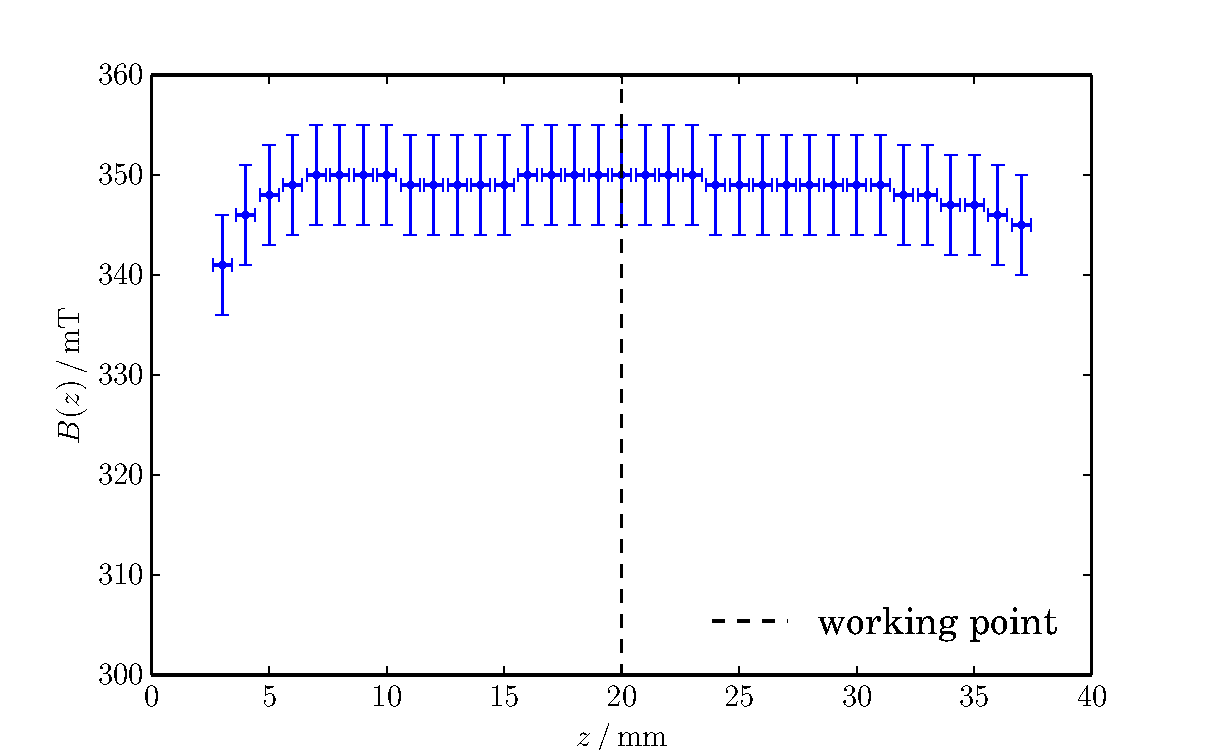
\includegraphics[width=\textwidth]{figures/b_height.pdf}
\caption{   
    Measurement of the homogenity of the unmodulated magnetic field $B$ in the vertical direction $z$. 
    The appied current is $I = 2.62$ A. As we observe a plateau between $z = 7$ mm and $z = 31$ mm, 
    we define the working point for the further experiments for $z = 20$ mm.
    For measured values, refer to table \ref{tab:b_height}.
    }
\label{fig:b_height}
\end{figure}
\FloatBarrier

\subsection{Dependency $B(I)$}
Measuring the magnetic fields of the main coil for different currents yielded two 
important results, which can be observed in figure \ref{fig:b_I}:
\begin{itemize}
\item
    In the regime $I < 3$ A, $B(I)$ behaves linear. We calculated fit parameters 
    for a least square fit using the corresponding routine 'numpy.polyfit'\ref{scipy} for 
    a first degree polynome $f(I) = p_0 I + p_1$ for the pairs $(I, B(I))$, $I \le 3.36$ A. 
    The resulting parameters $p_0$ and $p_1$ with covariance matrix are given by:
    \begin{align}
        p_0 &= 129 \pm 3 \mT / \A\\
        p_1 &= 16 \pm 7 \mT\\
        \mathrm{cov}(p_i, p_j) &= 
        \begin{pmatrix}
            11.1\frac{\mT^2}{\A^2} &-21.5\frac{\mT^2}{\A} \\
            -21.5\frac{\mT^2}{\A} &51.0\mT^2 \\
        \end{pmatrix} 
        \, \mathrm{}
    \end{align}
    The relative error 
    \begin{equation}
        \frac{\Delta p_0}{p_0} = 3 / 129 \approx 2\%
    \end{equation}
    indicates the linear behaviour in the chosen regime which is expected from the 
    graphical analysis. 
\item
    We observe a non-linear behaviour for $I > 3$ A. However, this regime is 
    not reached during the other measurements, so that we relinquish the further analysis. 
\end{itemize}
\begin{figure}
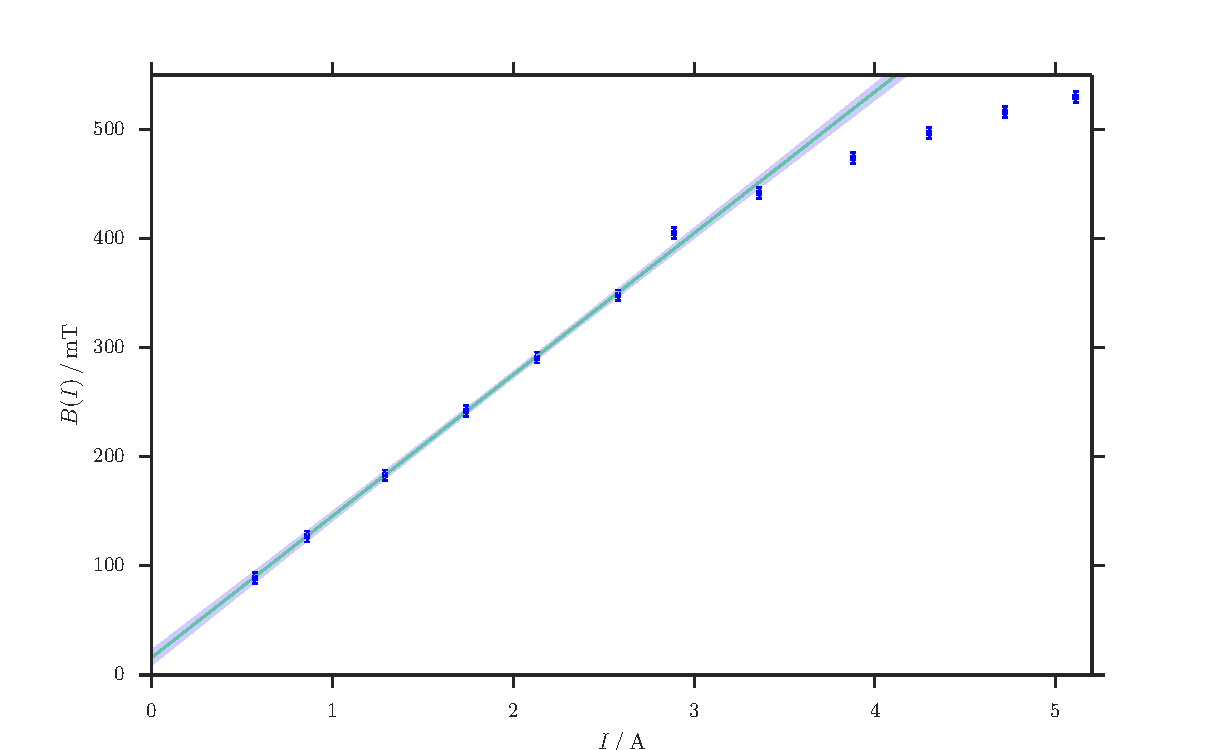
\includegraphics[width=\textwidth]{figures/b_I.pdf}
\caption{   
    Measurement of magnetic field $B$ of the main coil depending on the applied current 
    $I$ at the working point $z = 20$ mm. The error bars corresponding 
    to the uncertainties $\Delta I = 0.01$ A 
    and $\Delta B = 5$ mT are plotted but visibly very small at this scale. 
    The line is showing the least square fit for $f(I) = p_0 I + p_1$. The 
    lighter shade indicates the uncertainties calculated from the parameters 
    and the covariance matrix. 
    The measured values are shown in table \ref{tab:b_I}.
    }
\label{fig:b_I}
\end{figure}

